\section{Calcul des dérivées}

\subsection{Entraînement du PINNs sur $\Omega$ (cercle)}

\subsubsection{Prédiction sur $\Omega$}

\textbf{Dérivées premières :}

\begin{figure}[H]
	\centering
	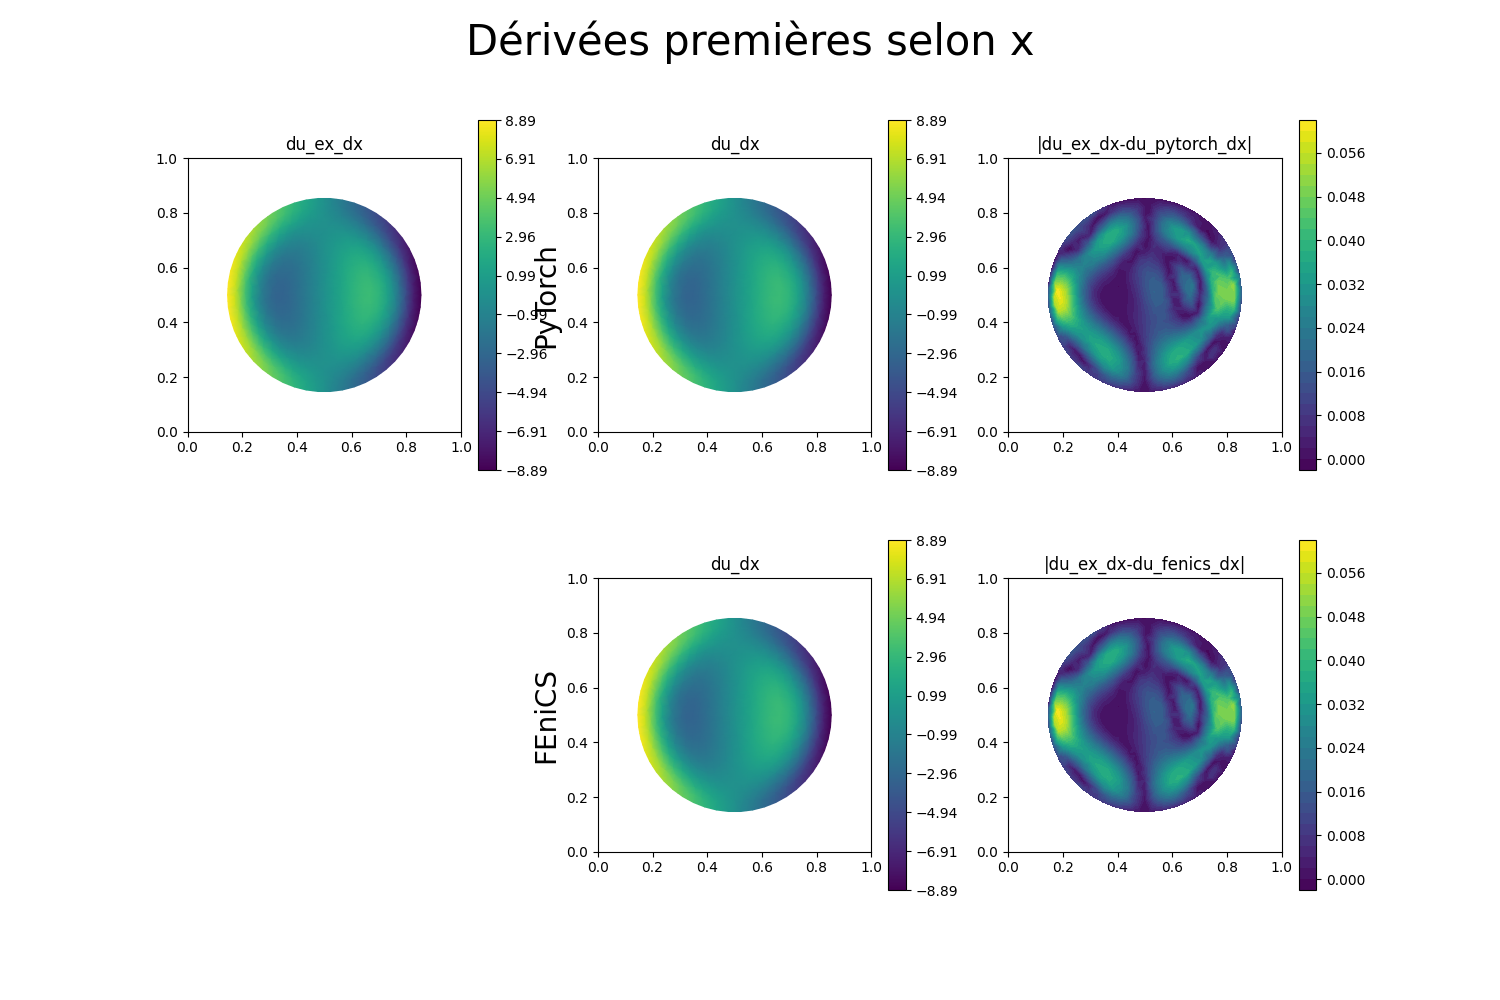
\includegraphics[width=0.75\linewidth]{derivees/derivees_circle_Omega_x}
	\label{fig:deriveescircleomegax}
\end{figure}

\begin{figure}[H]
	\centering
	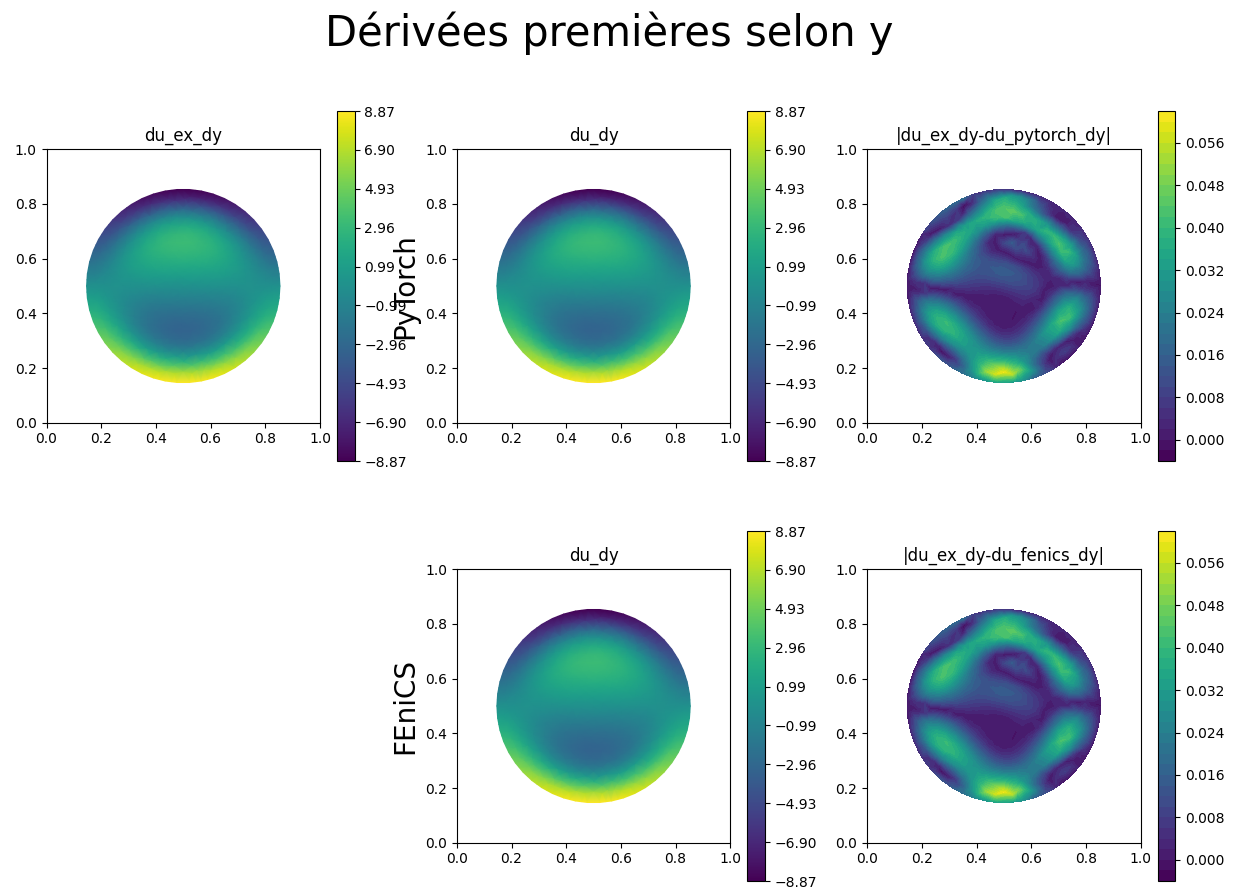
\includegraphics[width=0.75\linewidth]{derivees/derivees_circle_Omega_y}
	\label{fig:deriveescircleomegay}
\end{figure}

\newpage

\textbf{Dérivées secondes :}

\begin{figure}[H]
	\centering
	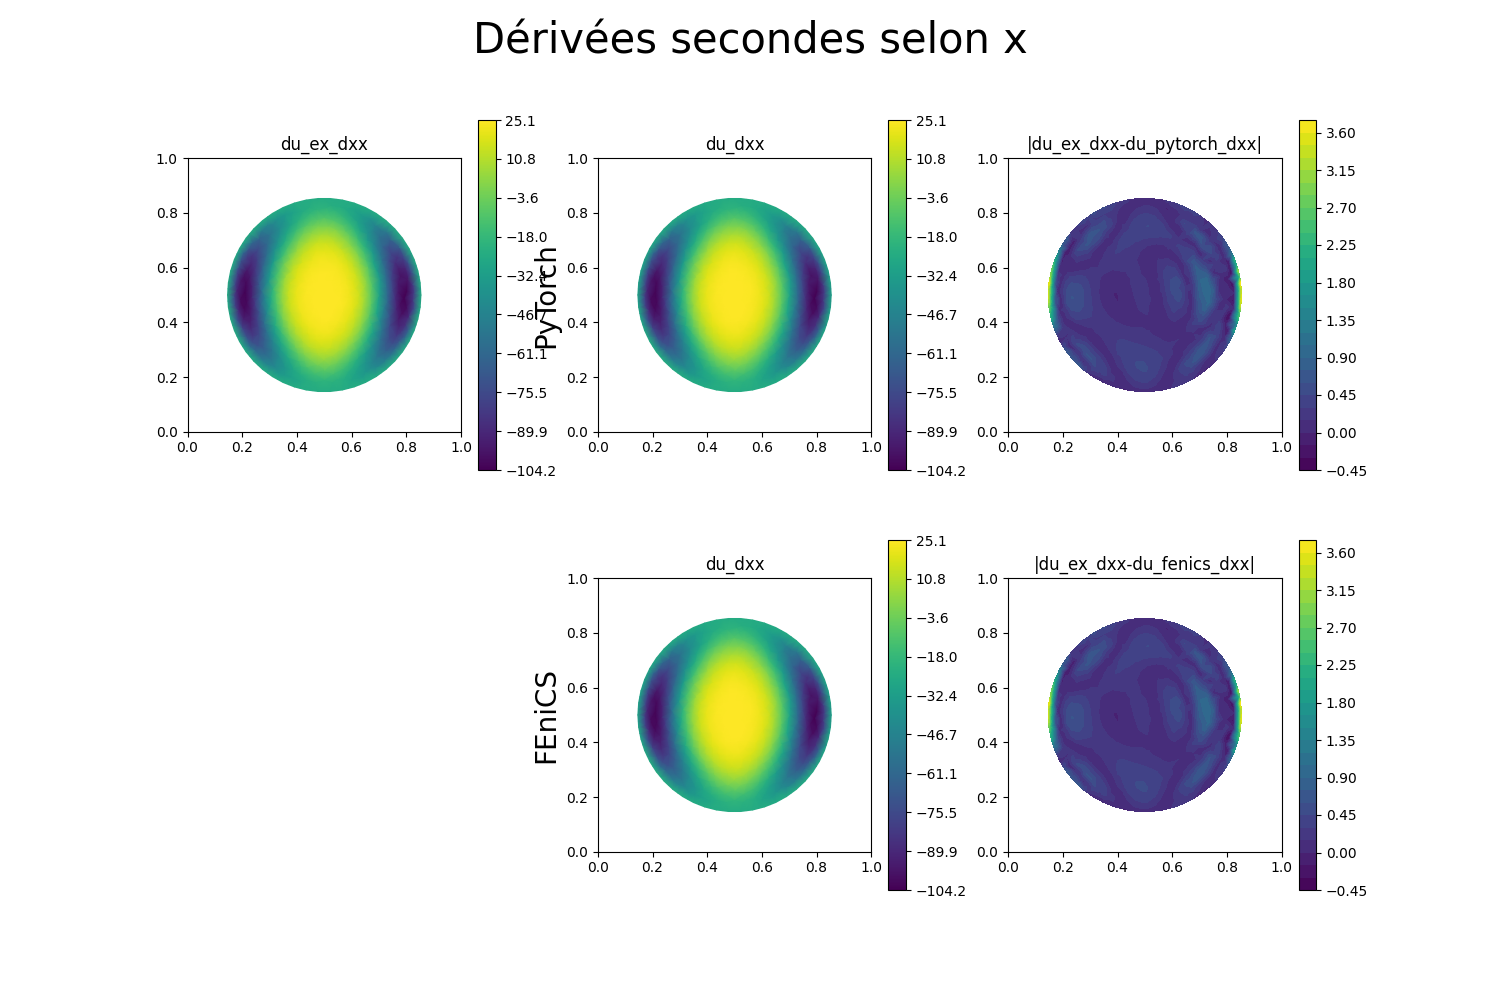
\includegraphics[width=0.85\linewidth]{derivees/derivees_circle_Omega_xx}
	\label{fig:deriveescircleomegaxx}
\end{figure}

\begin{figure}[H]
	\centering
	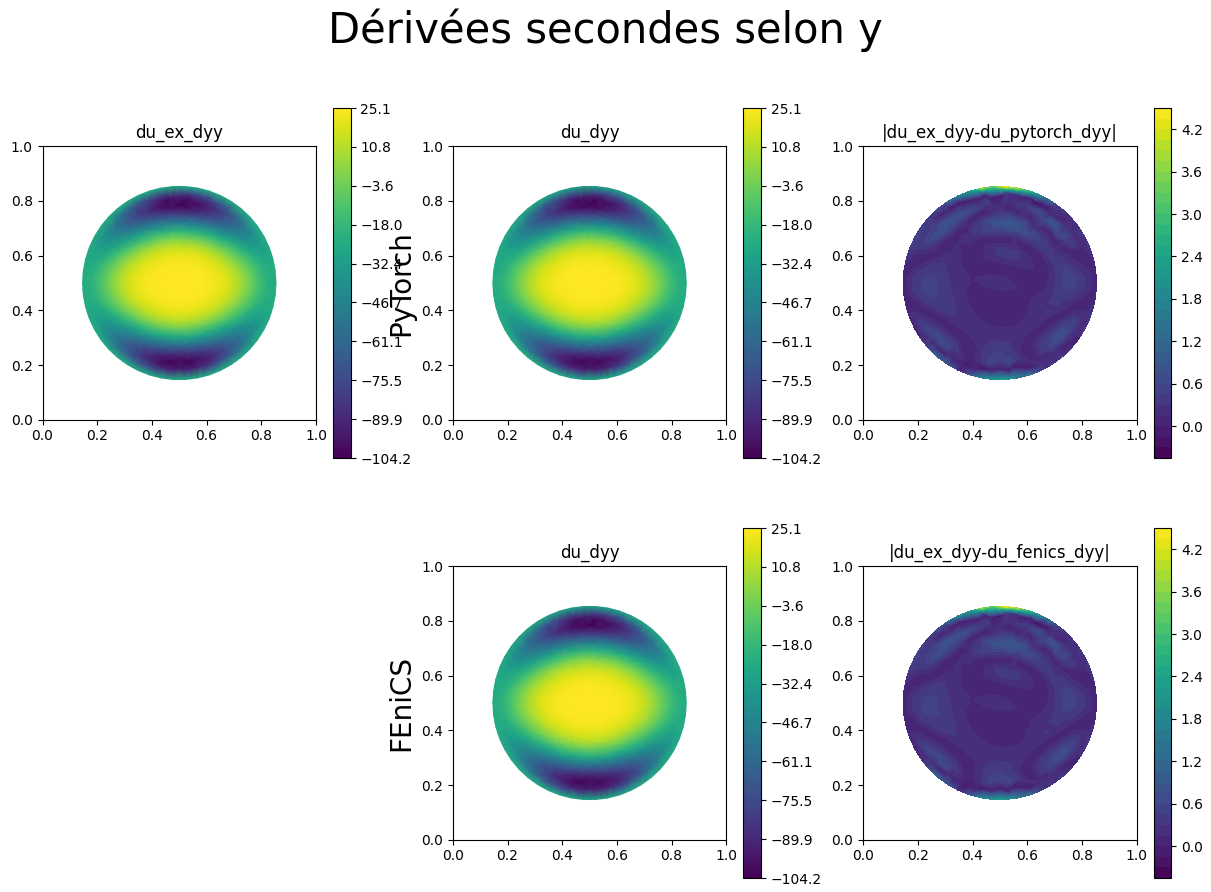
\includegraphics[width=0.85\linewidth]{derivees/derivees_circle_Omega_yy}
	\label{fig:deriveescircleomegayy}
\end{figure}

\newpage

\subsubsection{Prédiction sur $\Omega_h$}

\textbf{Dérivées premières :}

\begin{figure}[H]
	\centering
	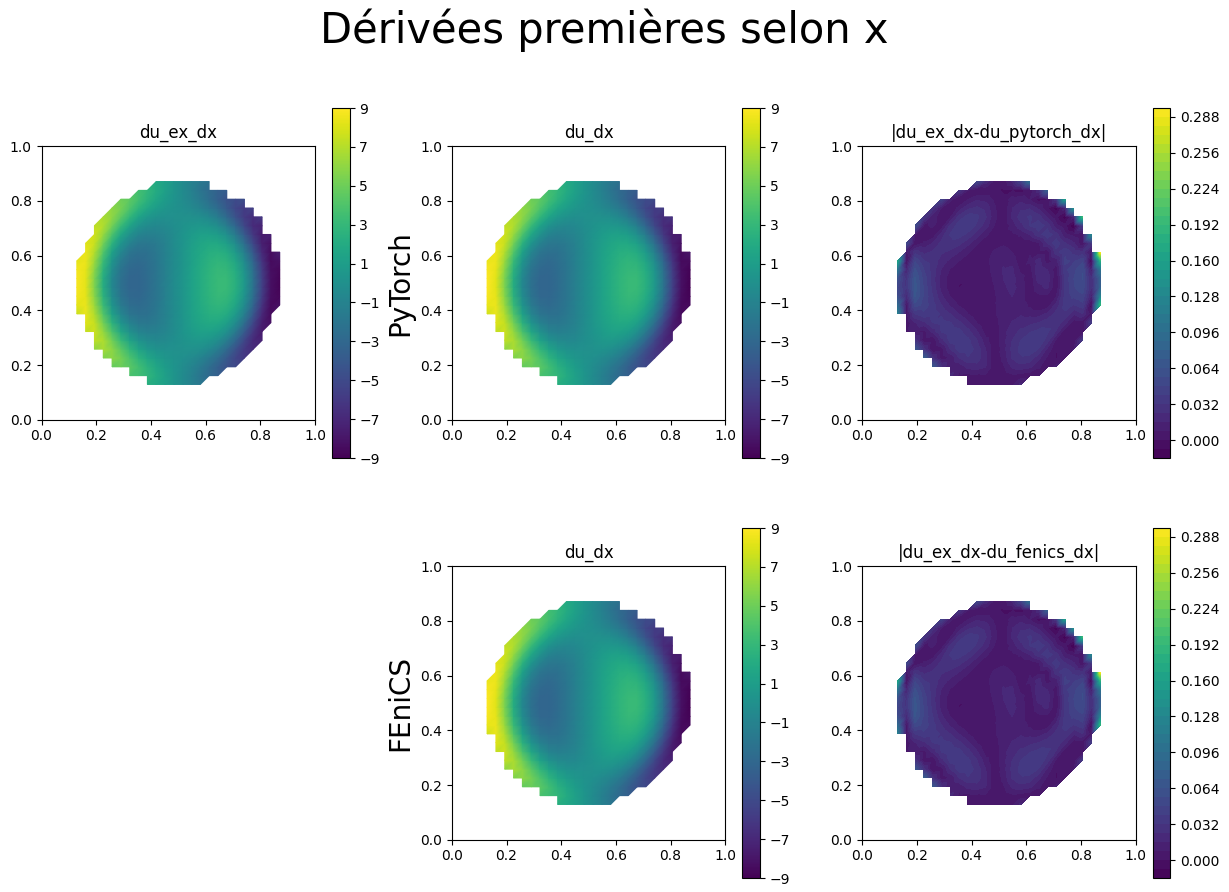
\includegraphics[width=0.85\linewidth]{derivees/derivees_circle_Omega_h_x}
	\label{fig:deriveescircleomegahx}
\end{figure}

\begin{figure}[H]
	\centering
	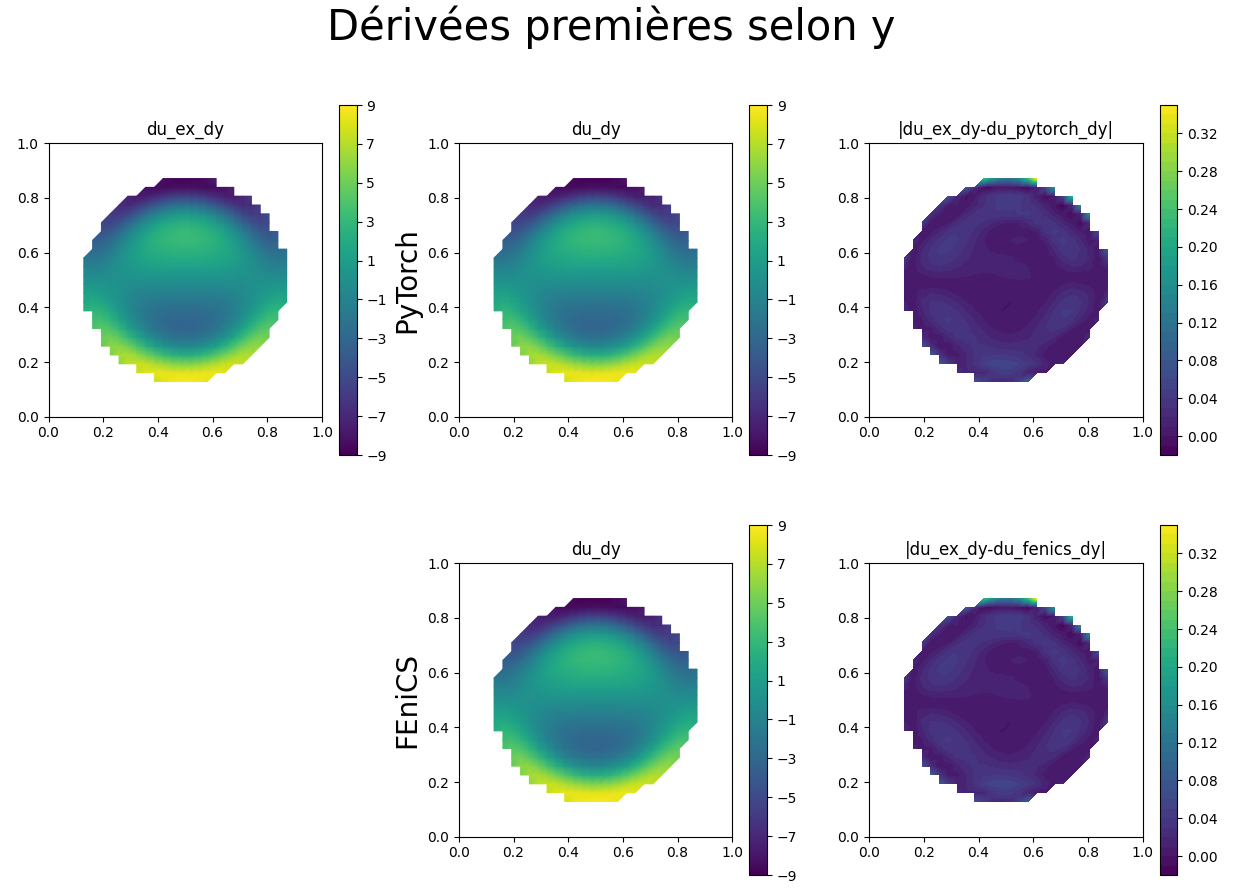
\includegraphics[width=0.85\linewidth]{derivees/derivees_circle_Omega_h_y}
	\label{fig:deriveescircleomegahy}
\end{figure}

\newpage

\textbf{Dérivées secondes :}

\begin{figure}[H]
	\centering
	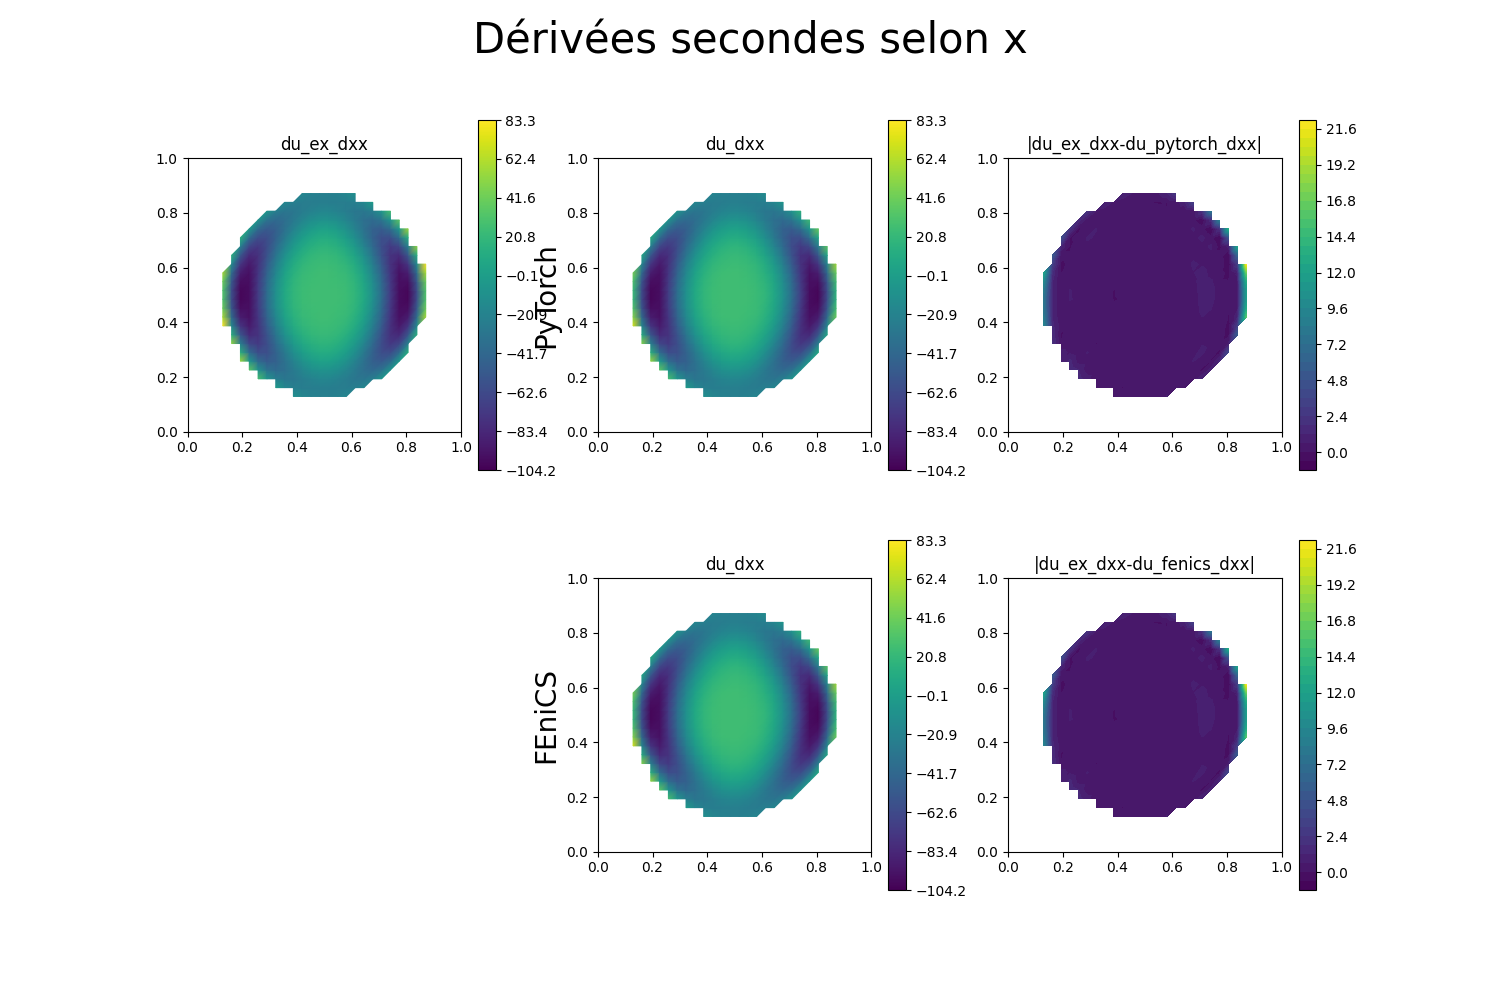
\includegraphics[width=0.85\linewidth]{derivees/derivees_circle_Omega_h_xx}
	\label{fig:deriveescircleomegahxx}
\end{figure}

\begin{figure}[H]
	\centering
	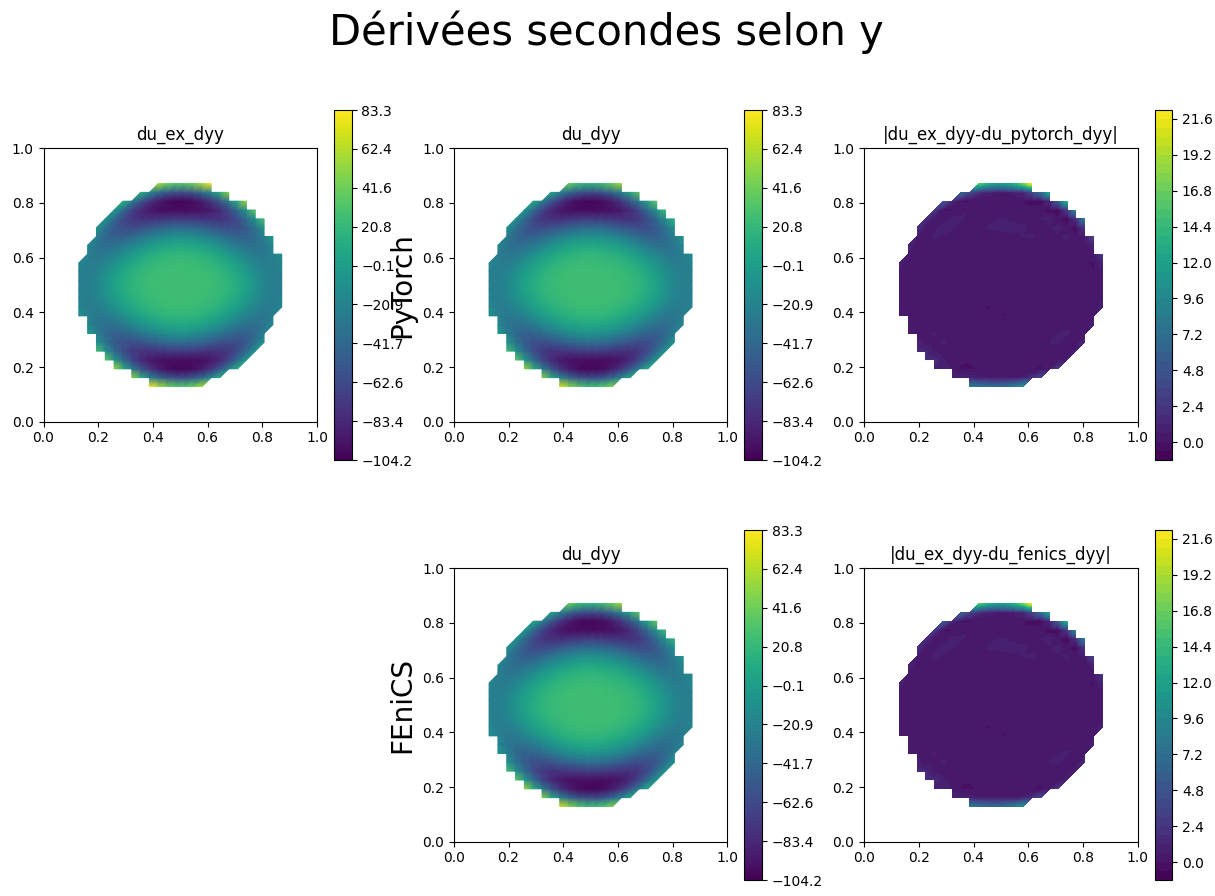
\includegraphics[width=0.85\linewidth]{derivees/derivees_circle_Omega_h_yy}
	\label{fig:deriveescircleomegahyy}
\end{figure}

\newpage

\subsection{Entraînement du PINNs sur $\mathcal{O}$ (carré)}

\subsubsection{Prédiction sur $\Omega$}

\textbf{Dérivées premières :}

\begin{figure}[H]
	\centering
	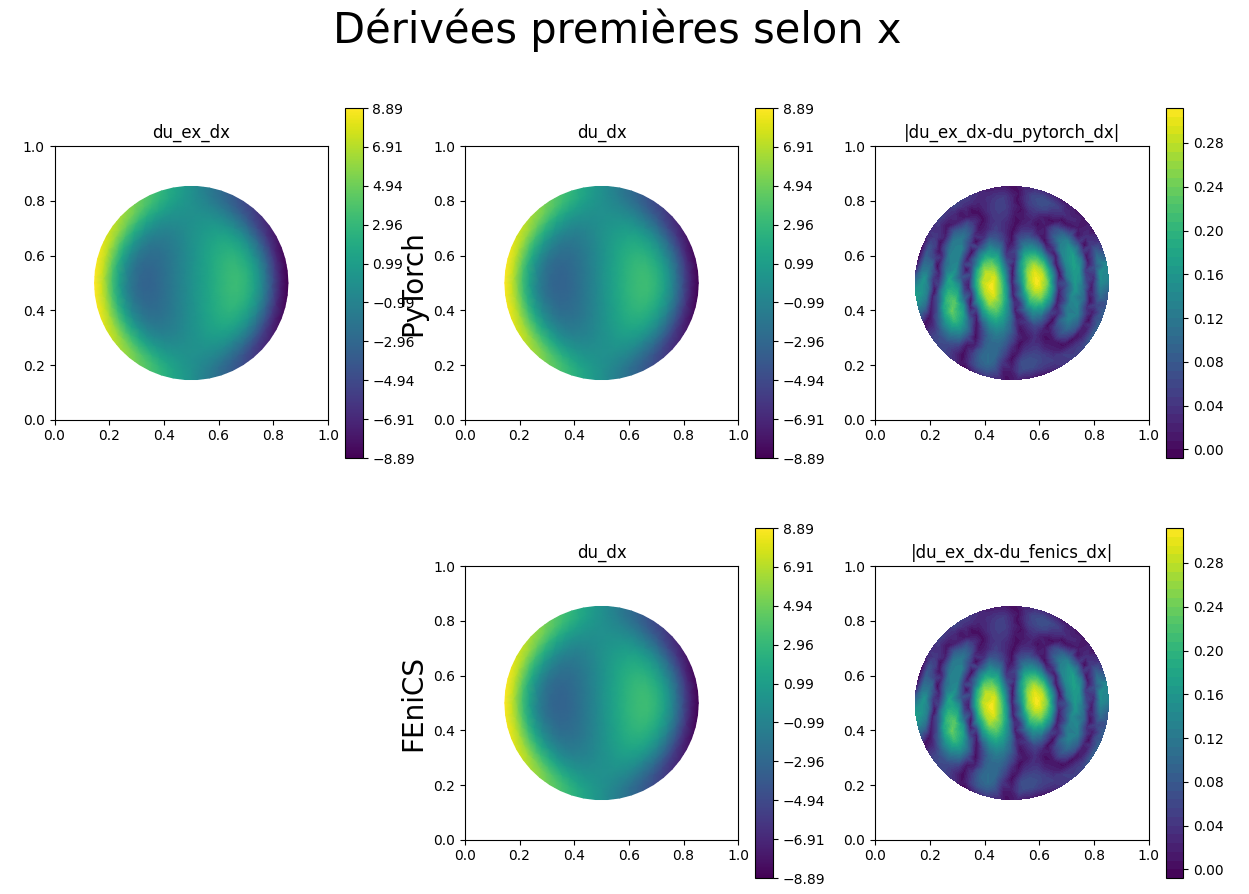
\includegraphics[width=0.8\linewidth]{derivees/derivees_square_Omega_x}
	\label{fig:deriveessquareomegax}
\end{figure}

\begin{figure}[H]
	\centering
	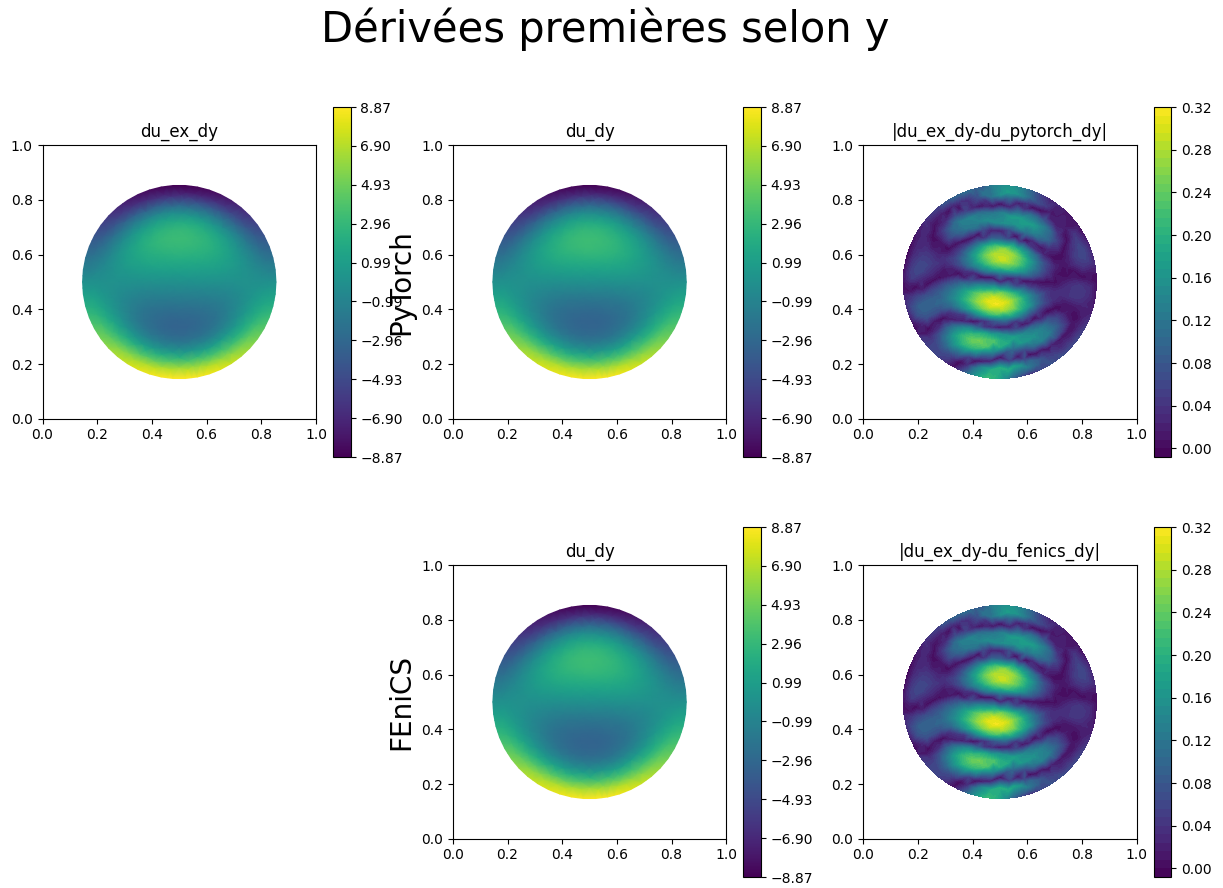
\includegraphics[width=0.8\linewidth]{derivees/derivees_square_Omega_y}
	\label{fig:deriveessquareomegay}
\end{figure}

\newpage

\textbf{Dérivées secondes :}

\begin{figure}[H]
	\centering
	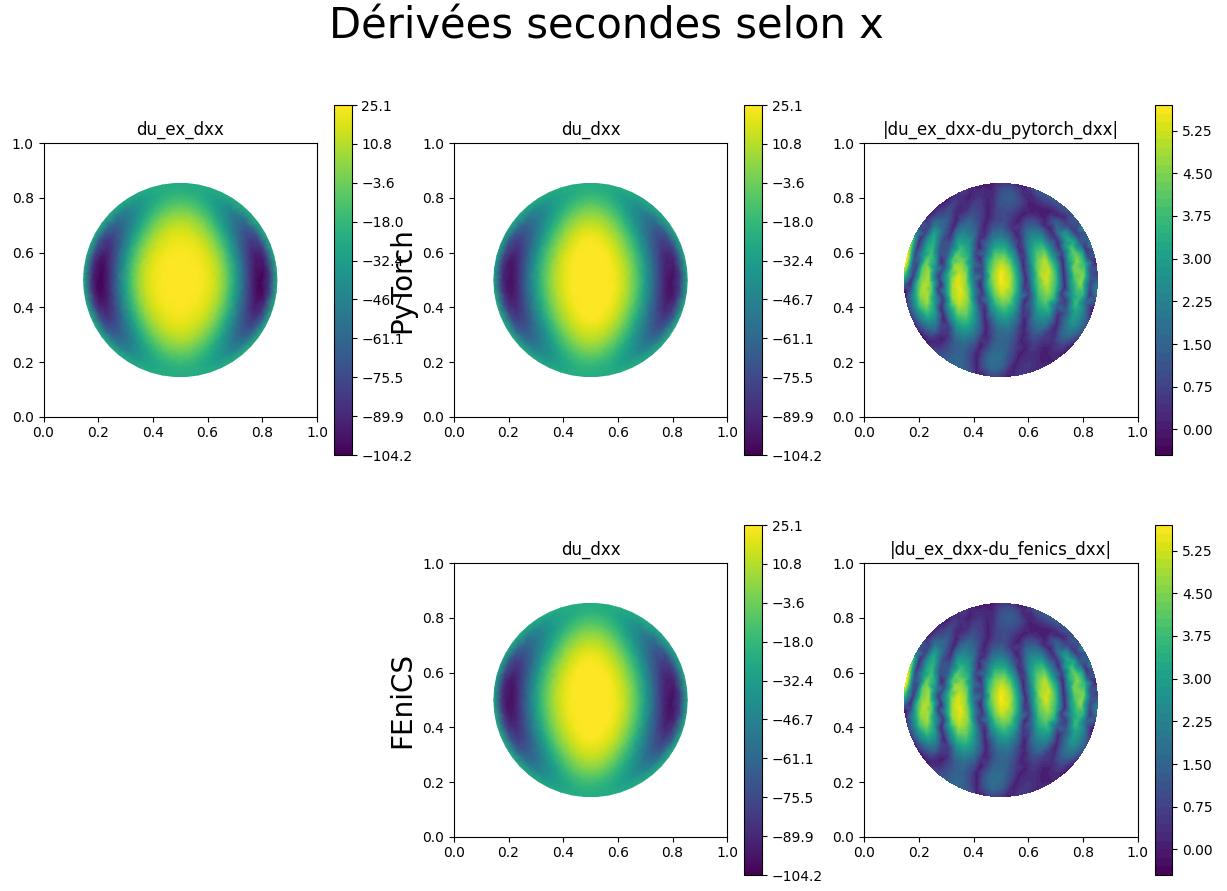
\includegraphics[width=0.85\linewidth]{derivees/derivees_square_Omega_xx}
	\label{fig:deriveessquareomegaxx}
\end{figure}

\begin{figure}[H]
	\centering
	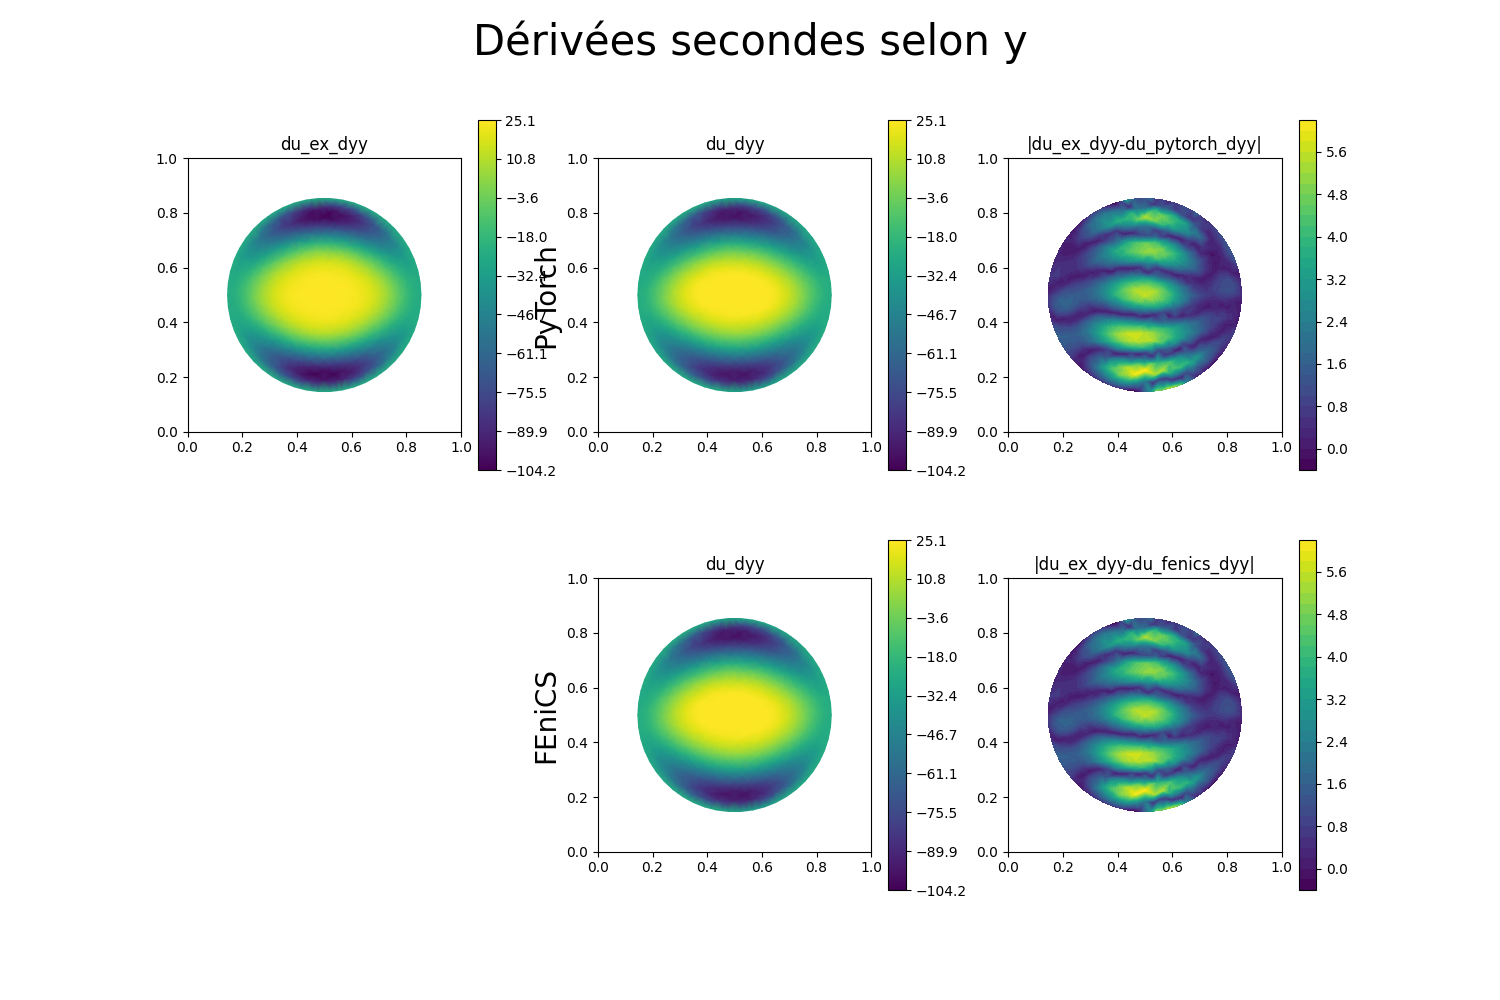
\includegraphics[width=0.85\linewidth]{derivees/derivees_square_Omega_yy}
	\label{fig:deriveessquareomegayy}
\end{figure}

\newpage

\subsubsection{Prédiction sur $\Omega_h$}

\textbf{Dérivées premières :}

\begin{figure}[H]
	\centering
	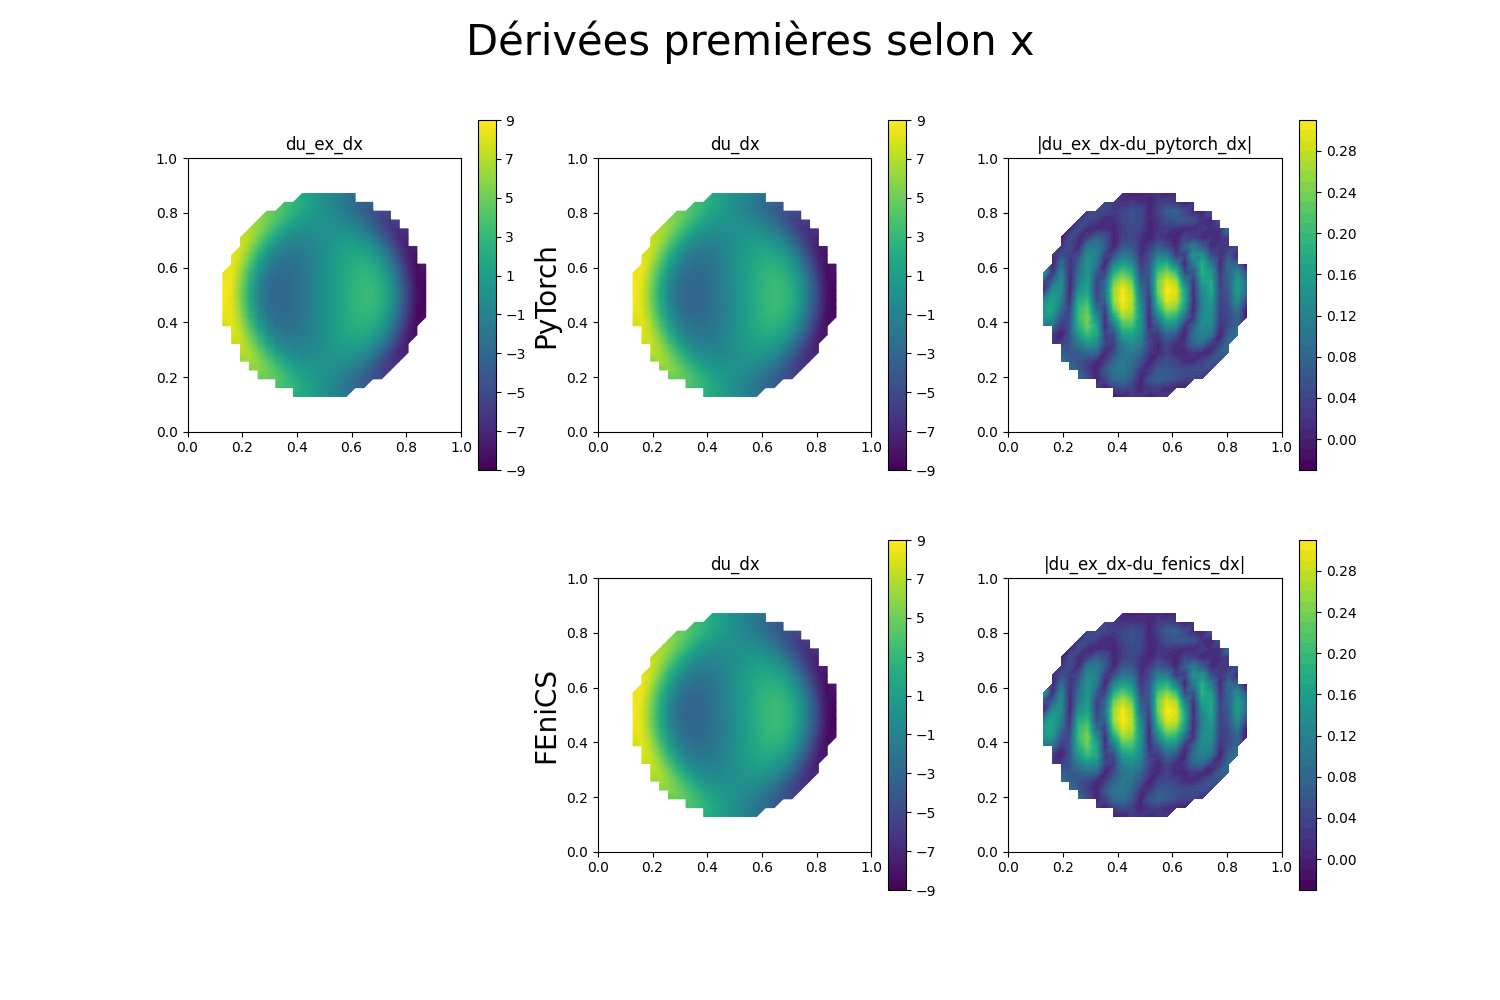
\includegraphics[width=0.85\linewidth]{derivees/derivees_square_Omega_h_x}
	\label{fig:deriveessquareomegahx}
\end{figure}

\begin{figure}[H]
	\centering
	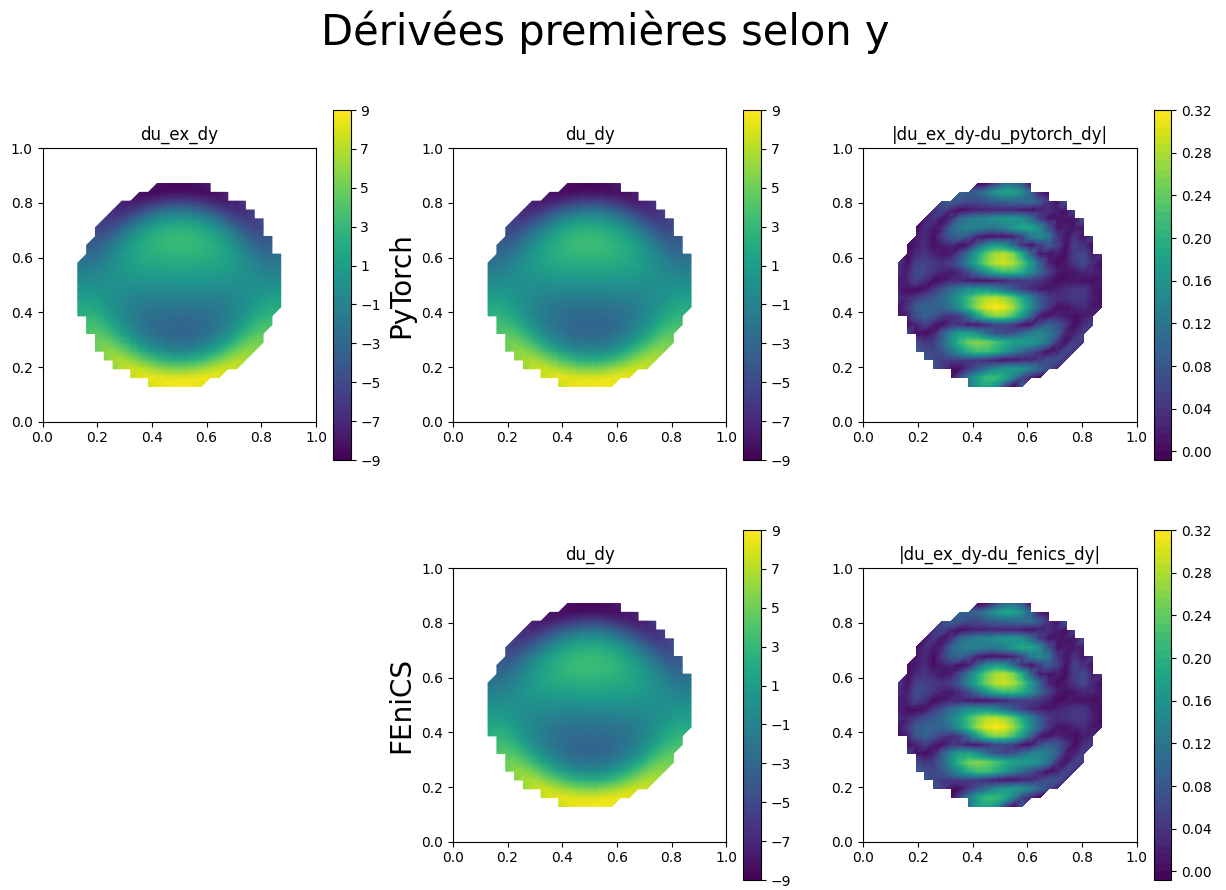
\includegraphics[width=0.85\linewidth]{derivees/derivees_square_Omega_h_y}
	\label{fig:deriveessquareomegahy}
\end{figure}

\newpage

\textbf{Dérivées secondes :}

\begin{figure}[H]
	\centering
	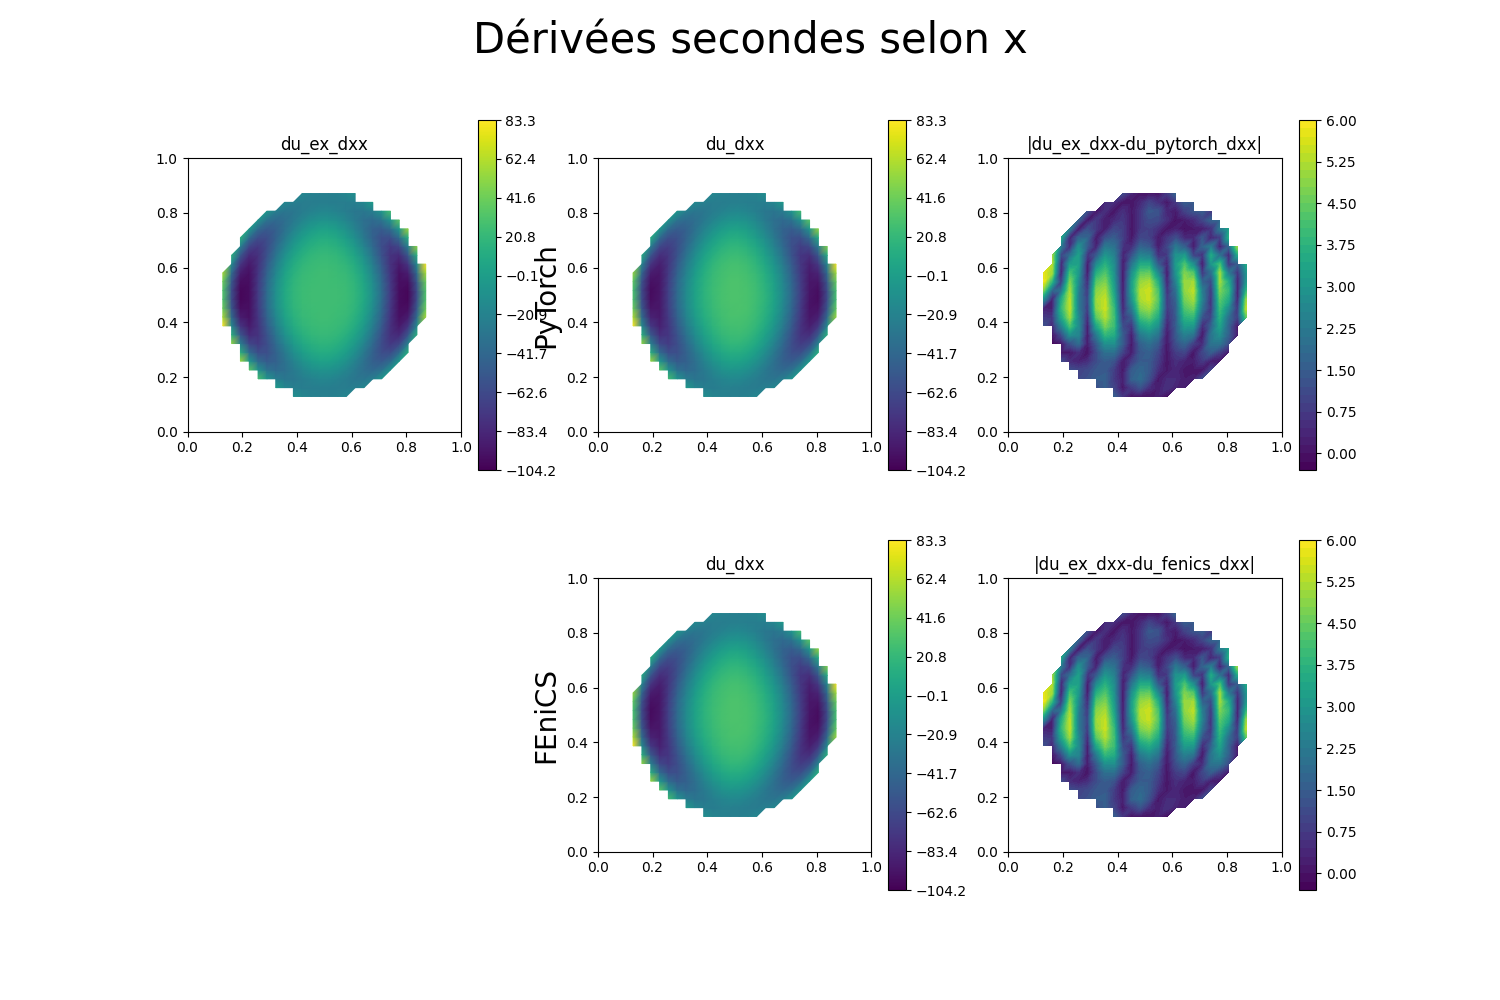
\includegraphics[width=0.85\linewidth]{derivees/derivees_square_Omega_h_xx}
	\label{fig:deriveessquareomegahxx}
\end{figure}

\begin{figure}[H]
	\centering
	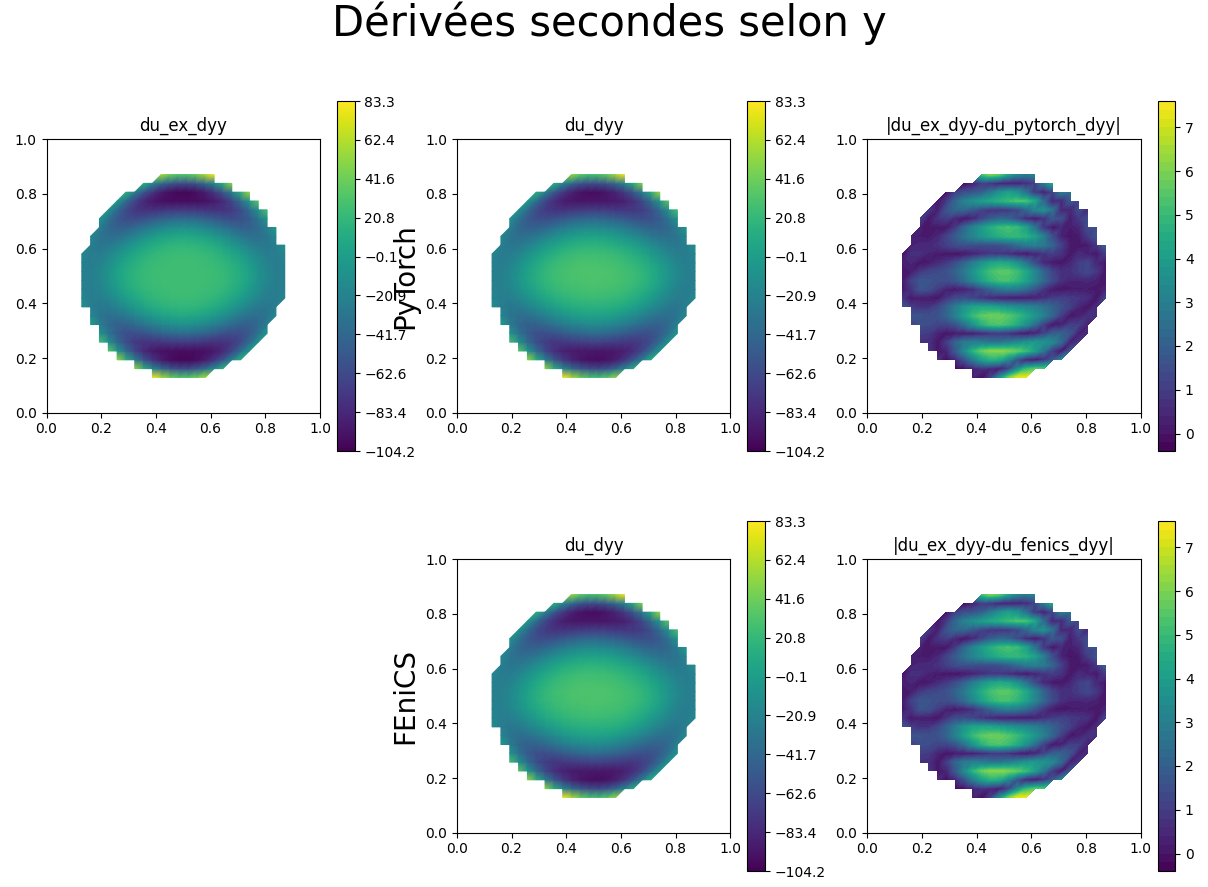
\includegraphics[width=0.85\linewidth]{derivees/derivees_square_Omega_h_yy}
	\label{fig:deriveessquareomegahyy}
\end{figure}

\newpage

\section{Test sur le degré de la solution exacte}

\begin{figure}[H]
	\centering
	\includegraphics[width=\linewidth]{degré}
	\label{fig:degre}
\end{figure}